\chapter{Preliminaries}\label{preliminaries}

\section{Reinforcement learning}\label{pl-rl}
RL, neural networks (incl non-linnear function approximation)

\section{State-space dimensionality reduction}\label{pl-dimensionality}
Definition, general info
Methods:
\subsection{Principal Component Analysis}\label{pl-pca}
algemene info pca
\subsection{Autoencoder}\label{pl-ae}
Another way of projecting data onto a lower dimensional space, is using an \emph{autoencoder}\cite{AE_general}. An autoencoder is a neural network consisting of two parts: an encoder network and a decoder network. The encoder projects the given input data onto a lower dimensional space, also called the \emph{latent space}. The output of the encoder, called the \emph{latent representation}, is used as input for the decoder. This decoder tries to reconstruct the original input from the latent representation as closely as possible. The autoencoder architecture is shown in figure \ref{fig:AE_architecture}.

\begin{figure}[h]
    \centering
    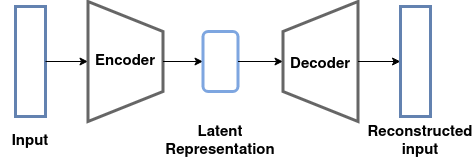
\includegraphics[width=0.75\textwidth]{AE_architecture}
    \caption{The architecture of an autoencoder.}
    \label{fig:AE_architecture}
\end{figure}

Formally, an autoencoder can be defined by the two functions it learns: 
\begin{equation}
  \label{enc}
  \phi :{\mathbb{R}^n}\rightarrow {\mathbb{R}^m}
\end{equation}
\begin{equation}
  \label{dec}
  \psi :{\mathbb{R}^m}\rightarrow {\mathbb{R}^n}
\end{equation}
\begin{equation}
  \label{encdec}
  \phi ,\psi ={\underset {\phi ,\psi }{\operatorname {arg\,min} }}\,{\Delta}(\psi \circ \phi (x))
\end{equation}
Equation~\eqref{enc} defines the encoder and equation~\eqref{dec} the decoder, both satisfying~\eqref{encdec} where $\Delta$ is the reconstruction loss function for input x.

A fundamental difference with using PCA, is the type of functions that can be approximated for lowering the dimensionality. Since an autoencoder uses neural networks, they can approximate nonlinear functions, as mentioned in section \ref{pl-rl}. This is in contrast with PCA, which can only approximate linear functions. Because of this, an autoencoder can learn more powerful generalisations which leads to lower information loss\cite{AE_general}.

\subsection{DeepMDP}\label{pl-deepmdp}
Info over deepmdp
